49. \begin{figure}[ht!]
\center{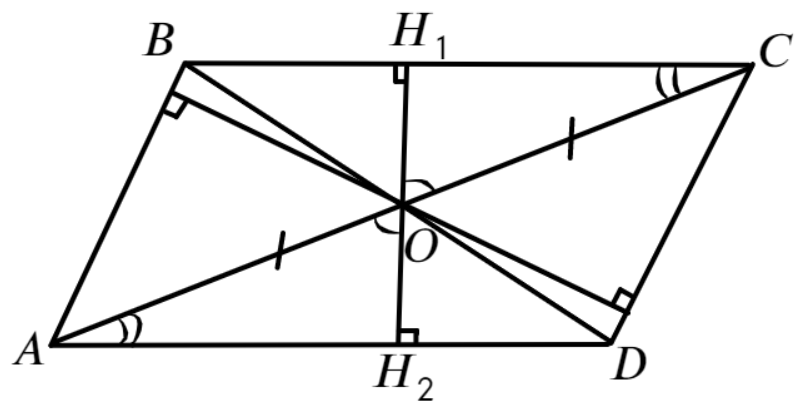
\includegraphics[scale=0.35]{g8-49.png}}
\end{figure}\\
Проведём перпендикуляры из точки пересечения диагоналей ко всем сторонам параллелограмма. Треугольники $AOH_2$ и $COH_1$ равны по второму признаку: $AO=OC,$ Углы $AOH_2$ и $COH_1$ вертикальные, а $H_2AO$ и $H_1CO$ --- накрест лежащие. Значит, $H_1O=H_2O,$ поэтому $H_1H_2=2OH_1.$ Поэтому высоты параллелограмма в два раза больше, чем расстояния от точки пересечения диагоналей до сторон. Тогда одна сторона равна $24:6=4$см, а другая $24:4=6$см, таким образом периметр параллелограмма равен $(4+6)\cdot2=20$см.\\
